\documentclass[10pt,a4paper]{article}
\usepackage[utf8]{inputenc}
\usepackage{amsmath}
\usepackage{amsfonts}
\usepackage{amssymb}
\usepackage{graphicx}
\graphicspath{ {./images/} }
\usepackage[margin=.5in]{geometry}
\usepackage{parskip}
\begin{document}

 \large Metadata of the code and data for:\\

\normalsize
Bates, J. M., Fidino, M., Nowak-Boyd, L., Strausberger, B. M., Schmidt, K. A., and Whelan, C. J. Climate change affects nesting phenology of midwestern birds: comparison of modern field records with historical records obtained from museum collections.\\\\
\begin{center}
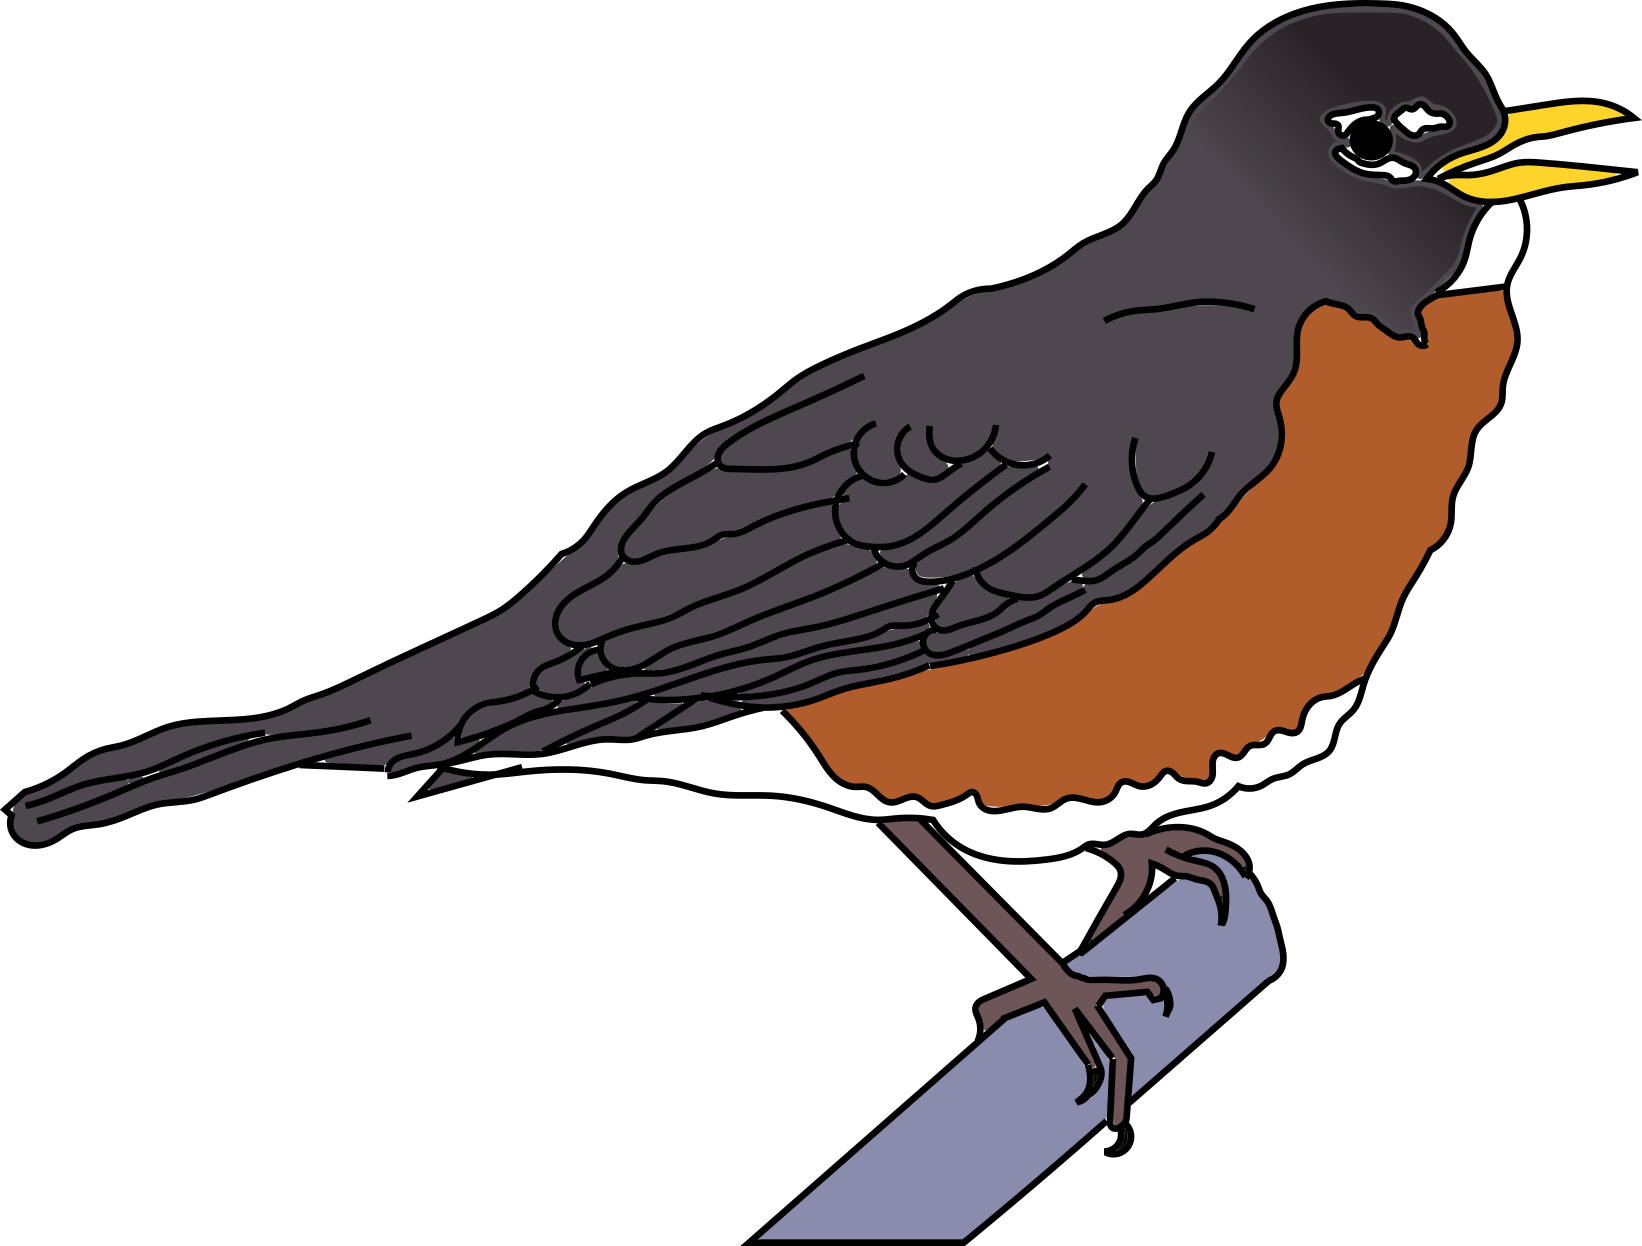
\includegraphics[width=0.15\textwidth]{american_robin.png}\\
\vspace{2mm}
\textbf{\Large Scripts}
\end{center}
\noindent\makebox[\linewidth]{\rule{\paperwidth}{0.4pt}}

\textbf{This repository has 3 R Scripts used for this analysis. They are within the working directory. They include:}\\

\begin{itemize}
\item  \textbf{\texttt{bates\_2017\_calc\_climate\_residuals.R:}} This script reads in the atmospheric CO2 data, fits a linear model to it (with year as the independent variable), and calculates the residuals.
These residuals are then used in our primary analysis.
\item \textbf{\texttt{bates\_2017\_analysis\_script.R:}} This script fits our robust to outlier model to bird nesting records.
\item \texttt{\textbf{bates\_2017\_plotting.R:}} This script can be used to generate the figures in the manuscript.
\end{itemize}
\vspace{3mm}
To conduct the analysis the scripts should be ran in the order listed above.\\
\noindent\makebox[\linewidth]{\rule{\paperwidth}{0.4pt}}

\begin{center}
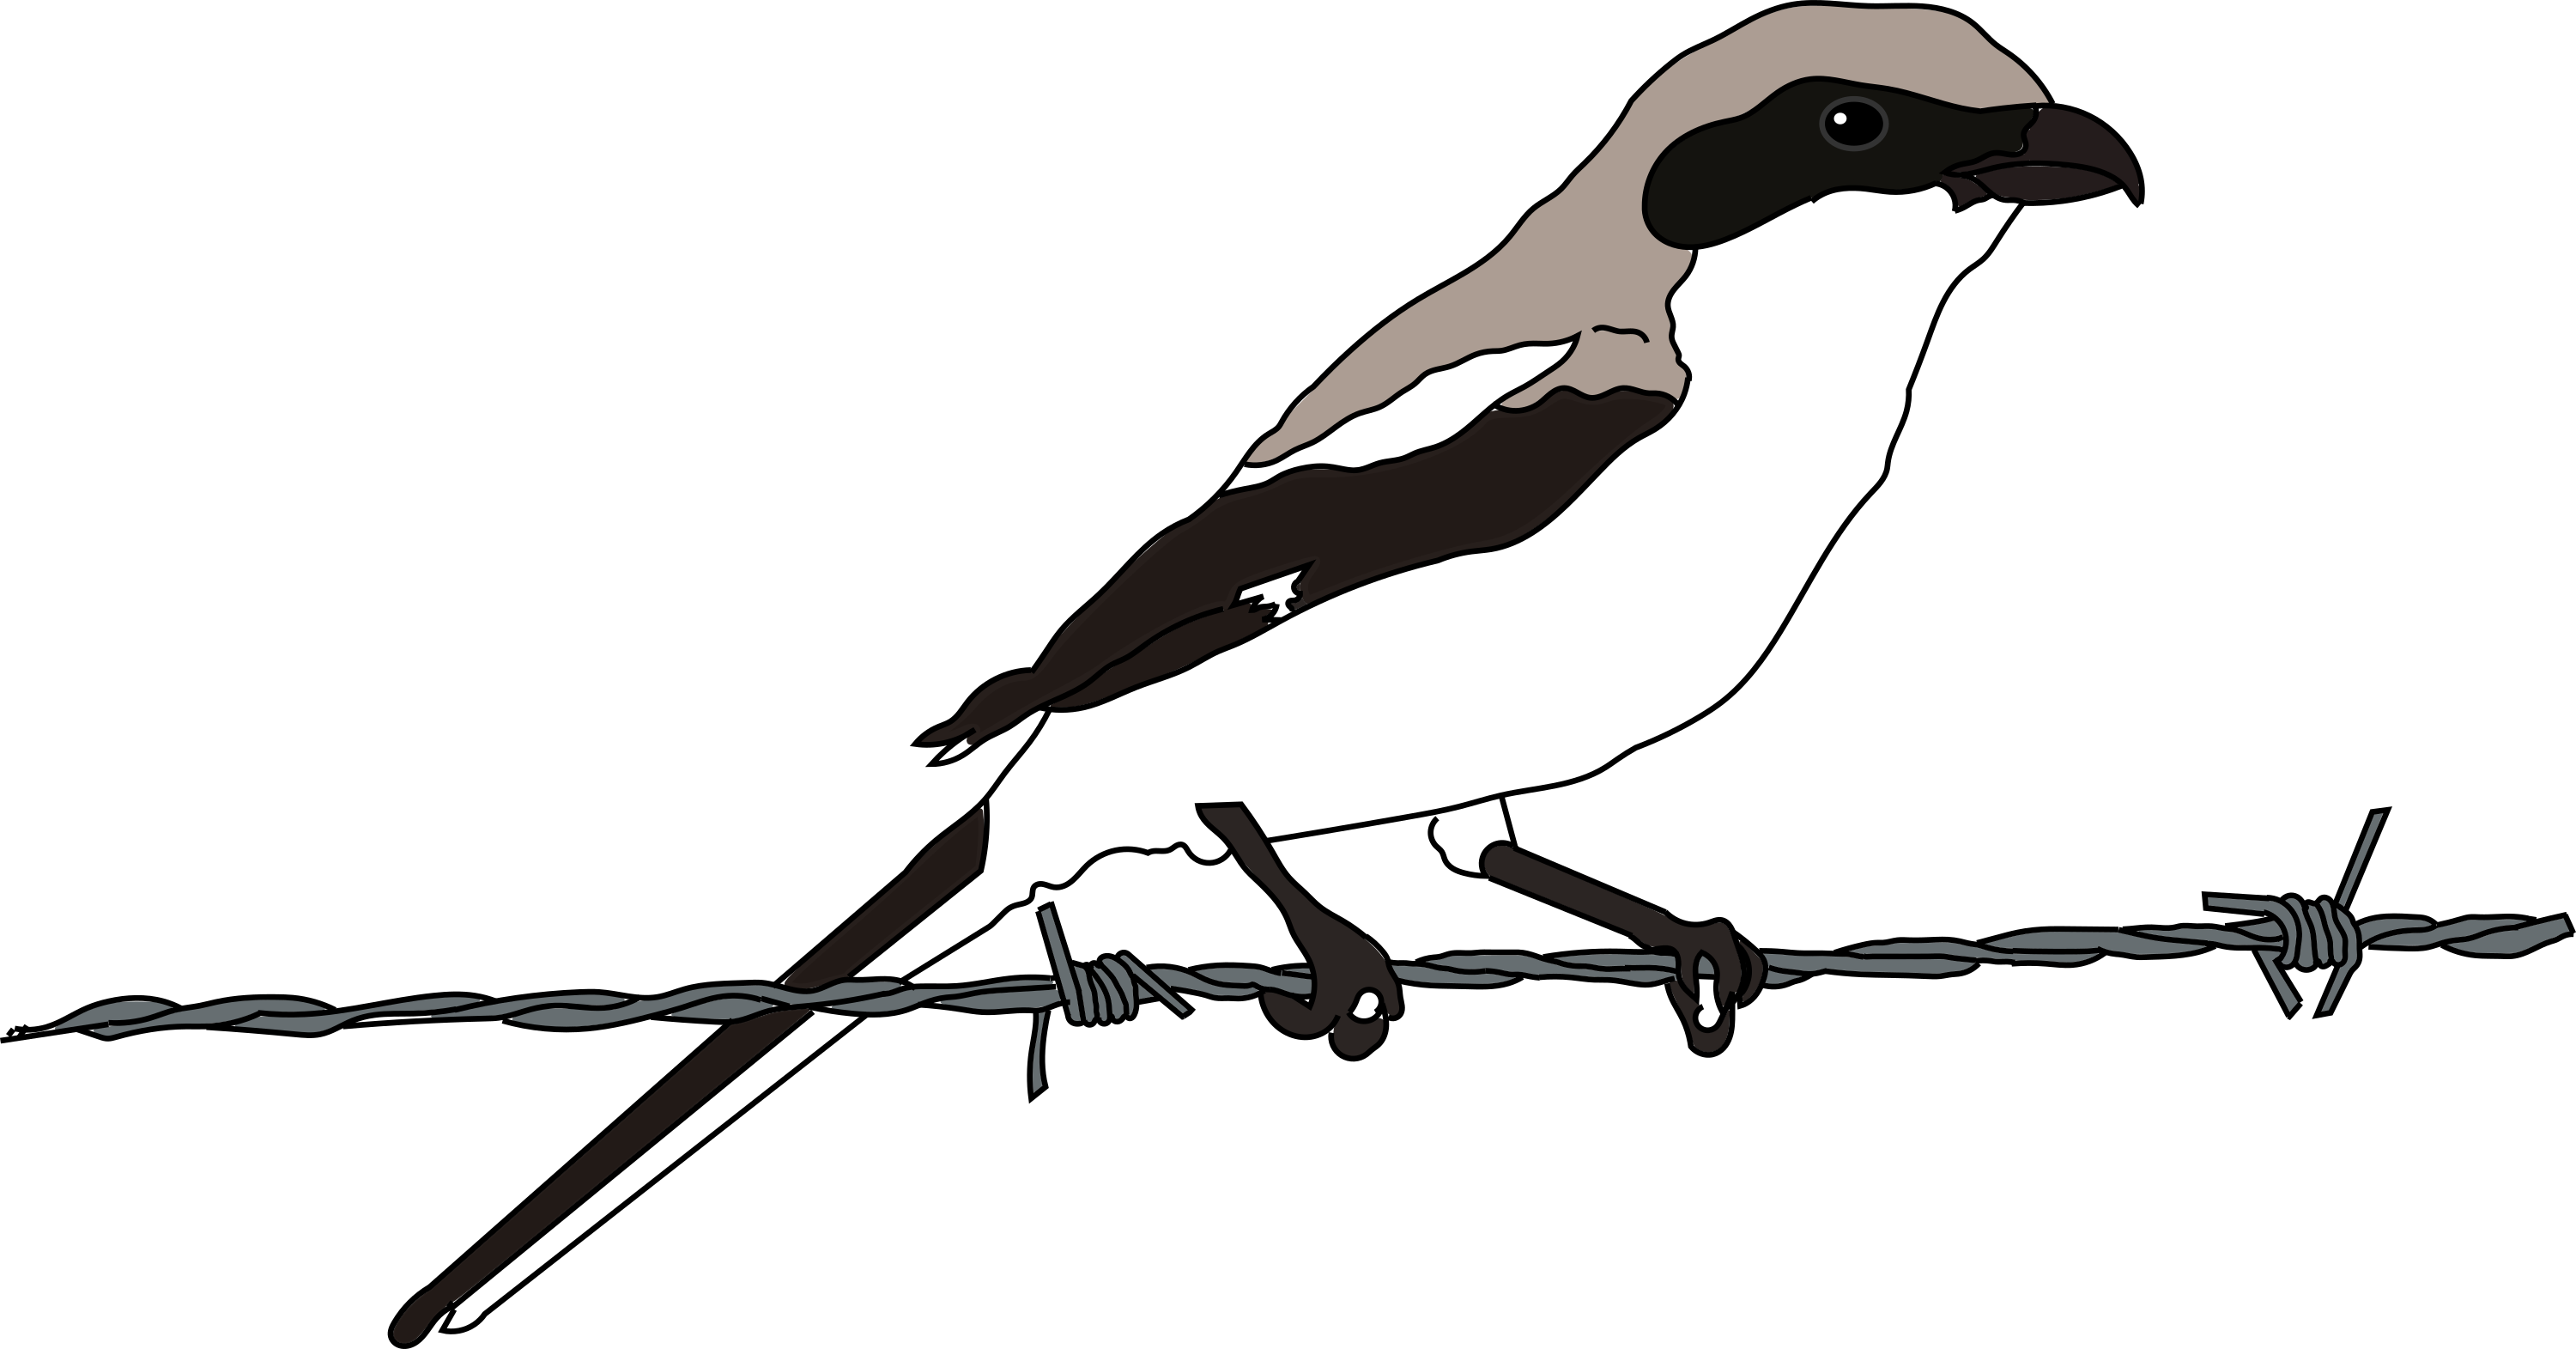
\includegraphics[width=0.15\textwidth]{shrike.png}\\
\vspace{2mm}
\textbf{\Large Models}
\end{center}
\noindent\makebox[\linewidth]{\rule{\paperwidth}{0.4pt}}


\textbf{This repository has 2 JAGS models that we used for our analysis. They should be placed within the jags\_models sub-folder of the working directory. These include:}\\

\begin{itemize}
\item \texttt{\textbf{bates\_2017\_climate\_resid\_model.R:}} This is the model that is called by \texttt{bates\_2017\_calc\_climate\_residuals.R}.
\item \texttt{\textbf{bates\_2017\_robust\_t\_model.R:}} This is the model that is called by \texttt{bates\_2017\_analysis\_script.R}. 
\end{itemize}

\noindent\makebox[\linewidth]{\rule{\paperwidth}{0.4pt}}

\begin{center}

\includegraphics[width=0.15\textwidth]{blue_jay.png}\\
\vspace{2mm}
\textbf{\Large Data}
\end{center}
\noindent\makebox[\linewidth]{\rule{\paperwidth}{0.4pt}}

\textbf{There are 3 data files within the data sub-folder which are used in this analysis. They include:}
\vspace{1.5mm}

\begin{itemize}
\item \texttt{bates\_2017\_co2.csv:} This is the global atmospheric CO2 levels per year. It contains 79 rows and 2 columns. \\The columns are:\\
\end{itemize}

\begin{center}
    \begin{tabular}{ | c | c | p{12cm} |}
    \hline
    Column header & Data type & Description\\
    \hline
     \texttt{yr}& Integer & The year the global atmospheric CO2 level is associated to. Ranges from 1744 to 2015. \\
     \hline
     \texttt{co2} & Numeric & The global atmospheric CO2 level on a given year.\\
    \hline
    \end{tabular}
\end{center}

Between 1744 and 1953, global CO2 levels were compiled from ice cores collected at Siple Station, West Antarctica (Neftel et al. 1994). 
For 1958 to 2015, direct observations of atmospheric CO2 levels were collected from the Mauna Loa Observatory (Keeling et al. 2008).

\textbf{References}

Keeling, RF, Piper, SC, Bollenbacher, AF, Walker, JS. 2008 Atmospheric CO2 Records from Sites in the Scripps Institution of Oceanography [SIO] Air Sampling Network [1985-2007]. Oak Ridge, TN (USA): Carbon Dioxide Information Analysis Center (CDIAC), Oak Ridge National Laboratory (ORNL).



Neftel, A, Friedli, H, Moor, E, Lötscher, H, Oeschger, H, Siegenthaler, U, Stauffer, B. 1994
Historical CO2 record from the Siple Station ice core. In Trends: A Compendium of Data on Global Change. Carbon Dioxide Information Analysis Center, Oak Ridge National Laboratory, Oak Ridge, Tenn., U.S.A., U.S. Department of Energy.

\vspace{1.5mm}

\begin{itemize}
\item \texttt{bates\_2017\_migratory\_status.csv:} These data relate a species to a specific migratory group as well as its American Ornithological Union (AOU) 4-letter alpha code. It has 72 rows of data and 3 columns. The columns are:\\
\end{itemize}

\begin{center}
    \begin{tabular}{ | c | c | p{12cm} |}
    \hline
    Column header & Data type & Description\\
    \hline
     \texttt{cmn}& Character & The common name of a given bird species. Species names are lowercase. \\
     \hline
     \texttt{migstat} & Character & The migratory status of a species. \texttt{long} indicates long-distance migrants (species that spend the non-breeding season primarily in the subtropics/tropics south of the United States border). \texttt{short} indicates short-distance migrants (species that spend the non-breeding season in southern temperate regions of the southern U.S.), and \texttt{resident} indicates permanent residents (species that maintain most of their populations in the study region throughout the year).\\
    \hline
    \texttt{species} & Character & The AOU 4-letter alpha code of a species.\\
    \hline
    \end{tabular}
\end{center}

 Migatory status for all species was compiled from https://www.allaboutbirds.org/
 
 \vspace{1.5mm}

\begin{itemize}
\item \texttt{bates\_2017\_bird\_lay\_dates.csv:} This is the lay date information for midwestern birds that were used in this analysis. It has 4958 rows and 4 columns. The columns are:
\end{itemize}

\begin{center}
    \begin{tabular}{ | c | c | p{12cm} |}
    \hline
    Column header & Data type & Description\\
    \hline
     \texttt{species}& Character & The AOU 4-letter alpha code of a species.\\
     \hline
     \texttt{jdate} & Integer & The julian date of the first lay date of a nest (Number of days from January 1 on a given year). \\
    \hline
    \texttt{year} & Integer &  The year the nest was found. \\
    \hline
    \texttt{period} & Categorical &  \texttt{low} indicates historic records housed at the Field museum of egg collections. \texttt{high} indicates current records of nest phenology collected through comprehensive field work by Chris Whelan and Bill Strausburger. \\
    \hline
    \end{tabular}
\end{center}


\begin{center}
\vspace{4mm}
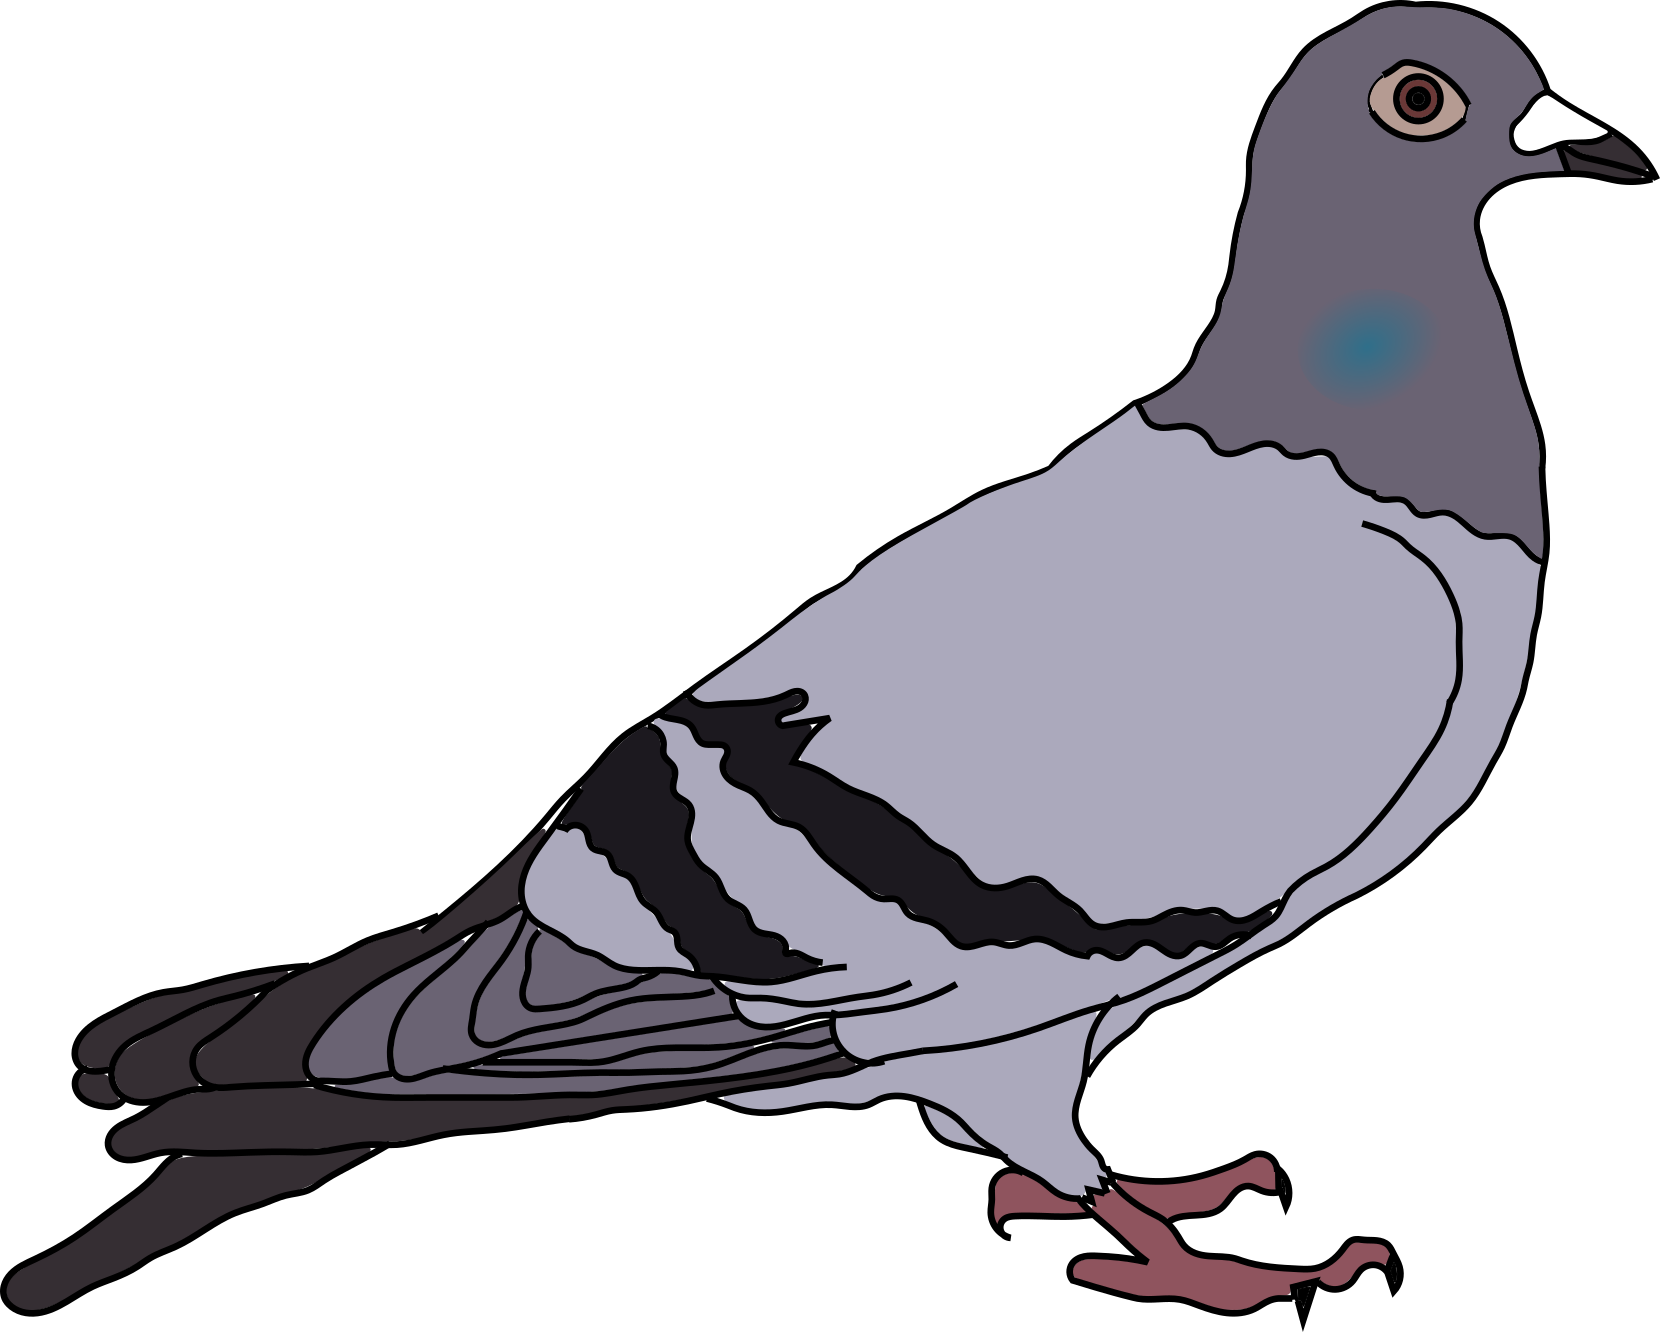
\includegraphics[width=0.15\textwidth]{rock_dove.png}
\end{center}


\end{document}